\hypertarget{stm32f4xx__hal__flash__ex_8c}{}\section{Dokumentacja pliku S\+T\+M/\+W\+D\+S\+\_\+\+Kosc\+\_\+\+Linux/\+Drivers/\+S\+T\+M32\+F4xx\+\_\+\+H\+A\+L\+\_\+\+Driver/\+Src/stm32f4xx\+\_\+hal\+\_\+flash\+\_\+ex.c}
\label{stm32f4xx__hal__flash__ex_8c}\index{S\+T\+M/\+W\+D\+S\+\_\+\+Kosc\+\_\+\+Linux/\+Drivers/\+S\+T\+M32\+F4xx\+\_\+\+H\+A\+L\+\_\+\+Driver/\+Src/stm32f4xx\+\_\+hal\+\_\+flash\+\_\+ex.\+c@{S\+T\+M/\+W\+D\+S\+\_\+\+Kosc\+\_\+\+Linux/\+Drivers/\+S\+T\+M32\+F4xx\+\_\+\+H\+A\+L\+\_\+\+Driver/\+Src/stm32f4xx\+\_\+hal\+\_\+flash\+\_\+ex.\+c}}


Extended F\+L\+A\+SH H\+AL module driver. This file provides firmware functions to manage the following functionalities of the F\+L\+A\+SH extension peripheral\+:  


{\ttfamily \#include \char`\"{}stm32f4xx\+\_\+hal.\+h\char`\"{}}\newline
Wykres zależności załączania dla stm32f4xx\+\_\+hal\+\_\+flash\+\_\+ex.\+c\+:\nopagebreak
\begin{figure}[H]
\begin{center}
\leavevmode
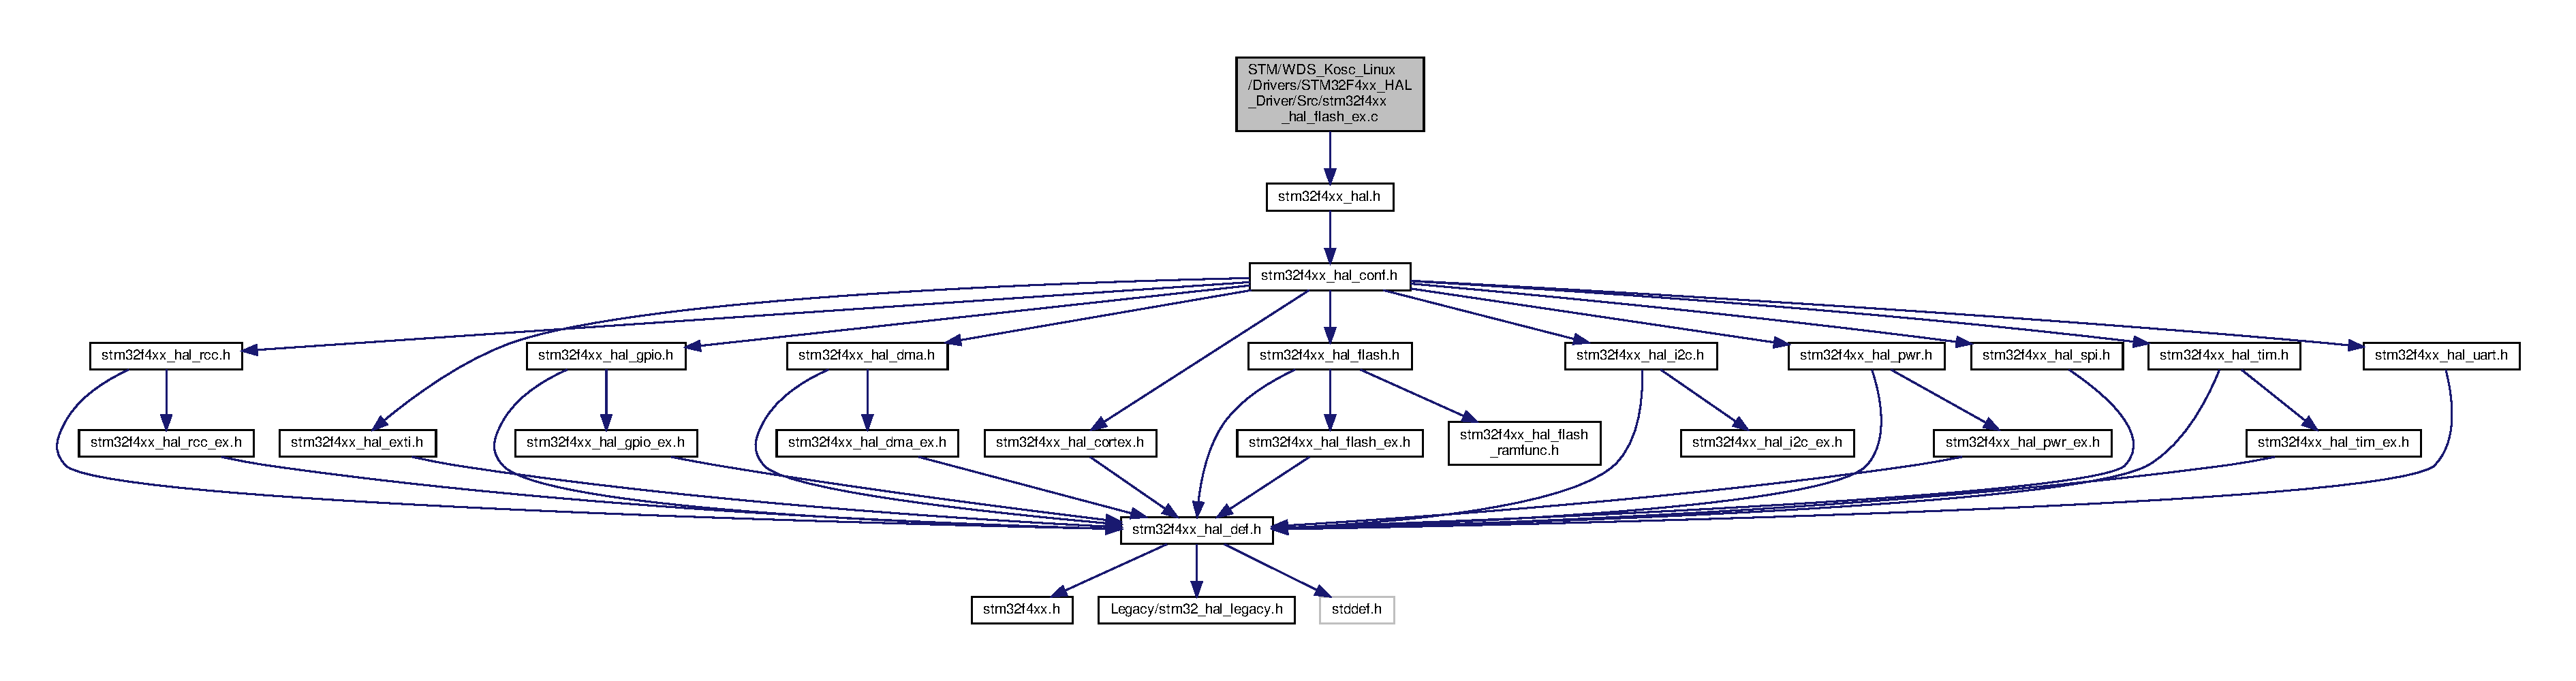
\includegraphics[width=350pt]{stm32f4xx__hal__flash__ex_8c__incl}
\end{center}
\end{figure}


\subsection{Opis szczegółowy}
Extended F\+L\+A\+SH H\+AL module driver. This file provides firmware functions to manage the following functionalities of the F\+L\+A\+SH extension peripheral\+: 

\begin{DoxyAuthor}{Autor}
M\+CD Application Team
\begin{DoxyItemize}
\item Extended programming operations functions
\end{DoxyItemize}
\end{DoxyAuthor}
\begin{DoxyVerb}==============================================================================
                 ##### Flash Extension features #####
==============================================================================
         
[..] Comparing to other previous devices, the FLASH interface for STM32F427xx/437xx and 
     STM32F429xx/439xx devices contains the following additional features 
     
     (+) Capacity up to 2 Mbyte with dual bank architecture supporting read-while-write
         capability (RWW)
     (+) Dual bank memory organization       
     (+) PCROP protection for all banks
 
                    ##### How to use this driver #####
==============================================================================
[..] This driver provides functions to configure and program the FLASH memory 
     of all STM32F427xx/437xx, STM32F429xx/439xx, STM32F469xx/479xx and STM32F446xx 
     devices. It includes
    (#) FLASH Memory Erase functions: 
         (++) Lock and Unlock the FLASH interface using HAL_FLASH_Unlock() and 
              HAL_FLASH_Lock() functions
         (++) Erase function: Erase sector, erase all sectors
         (++) There are two modes of erase :
           (+++) Polling Mode using HAL_FLASHEx_Erase()
           (+++) Interrupt Mode using HAL_FLASHEx_Erase_IT()
           
    (#) Option Bytes Programming functions: Use HAL_FLASHEx_OBProgram() to :
         (++) Set/Reset the write protection
         (++) Set the Read protection Level
         (++) Set the BOR level
         (++) Program the user Option Bytes
    (#) Advanced Option Bytes Programming functions: Use HAL_FLASHEx_AdvOBProgram() to :  
     (++) Extended space (bank 2) erase function
     (++) Full FLASH space (2 Mo) erase (bank 1 and bank 2)
     (++) Dual Boot activation
     (++) Write protection configuration for bank 2
     (++) PCROP protection configuration and control for both banks\end{DoxyVerb}


\begin{DoxyAttention}{Uwaga}

\end{DoxyAttention}
\subsubsection*{\begin{center}\copyright{} Copyright (c) 2017 S\+T\+Microelectronics. All rights reserved.\end{center} }

This software component is licensed by ST under B\+SD 3-\/\+Clause license, the \char`\"{}\+License\char`\"{}; You may not use this file except in compliance with the License. You may obtain a copy of the License at\+: opensource.\+org/licenses/\+B\+S\+D-\/3-\/\+Clause 